Als Kamera für die Objekterkennung wurde das Raspberry Pi Kamera Modul ausgewählt. Diese Kamera lässt sich über die CSI\footnote{Camera Serial Interface}-Schnittstelle direkt an den Raspberry Pi anschliessen. Die Bedienung der Kamera auf dem Raspberry Pi ist durch das Kommandozeilen-Programm \verb|raspistill| sehr komfortabel. Der einzige Nachteil ist der fixe Fokus der Kamera. Die Kamera besitzt jedoch eine Weitwinkel-Linse, mit welcher alle Gegenstände die weiter als eineinhalb Meter scharf dargestellt werden. Da das Spielfeld zwei Meter lang ist passt diese Distanz optimal zu den Anforderungen. Die Kamera hat ein horizontales Sichtfeld von $53^\circ$ und ein vertikales Sichtfeld von $40^\circ$. Für eine Distanz von zwei Meter entspricht das einer Fläche von 2×1.3 Meter, welche von der Kamera aufgenommen wird. Die detaillierte Berechnung kann dem Abschnitt \ref{subsub:sichtfeld-der-kamera} entnommen werden. Neben zahlreichen Einstellmöglichkeiten, fällt vor allem die kompakte Bauweise der Kamera auf (20×25×10 mm). Abbildung \ref{fig:raspberry_pi_cam} zeigt die Kamera mit dem mitgelieferten Anschlusskabel. Durch die oben genannten Eigenschaften eignet sich diese Kamera optimal für dieses Projekt und erfüllt auch alle erwarteten Anforderungen.

\begin{figure}[h!]
\centering
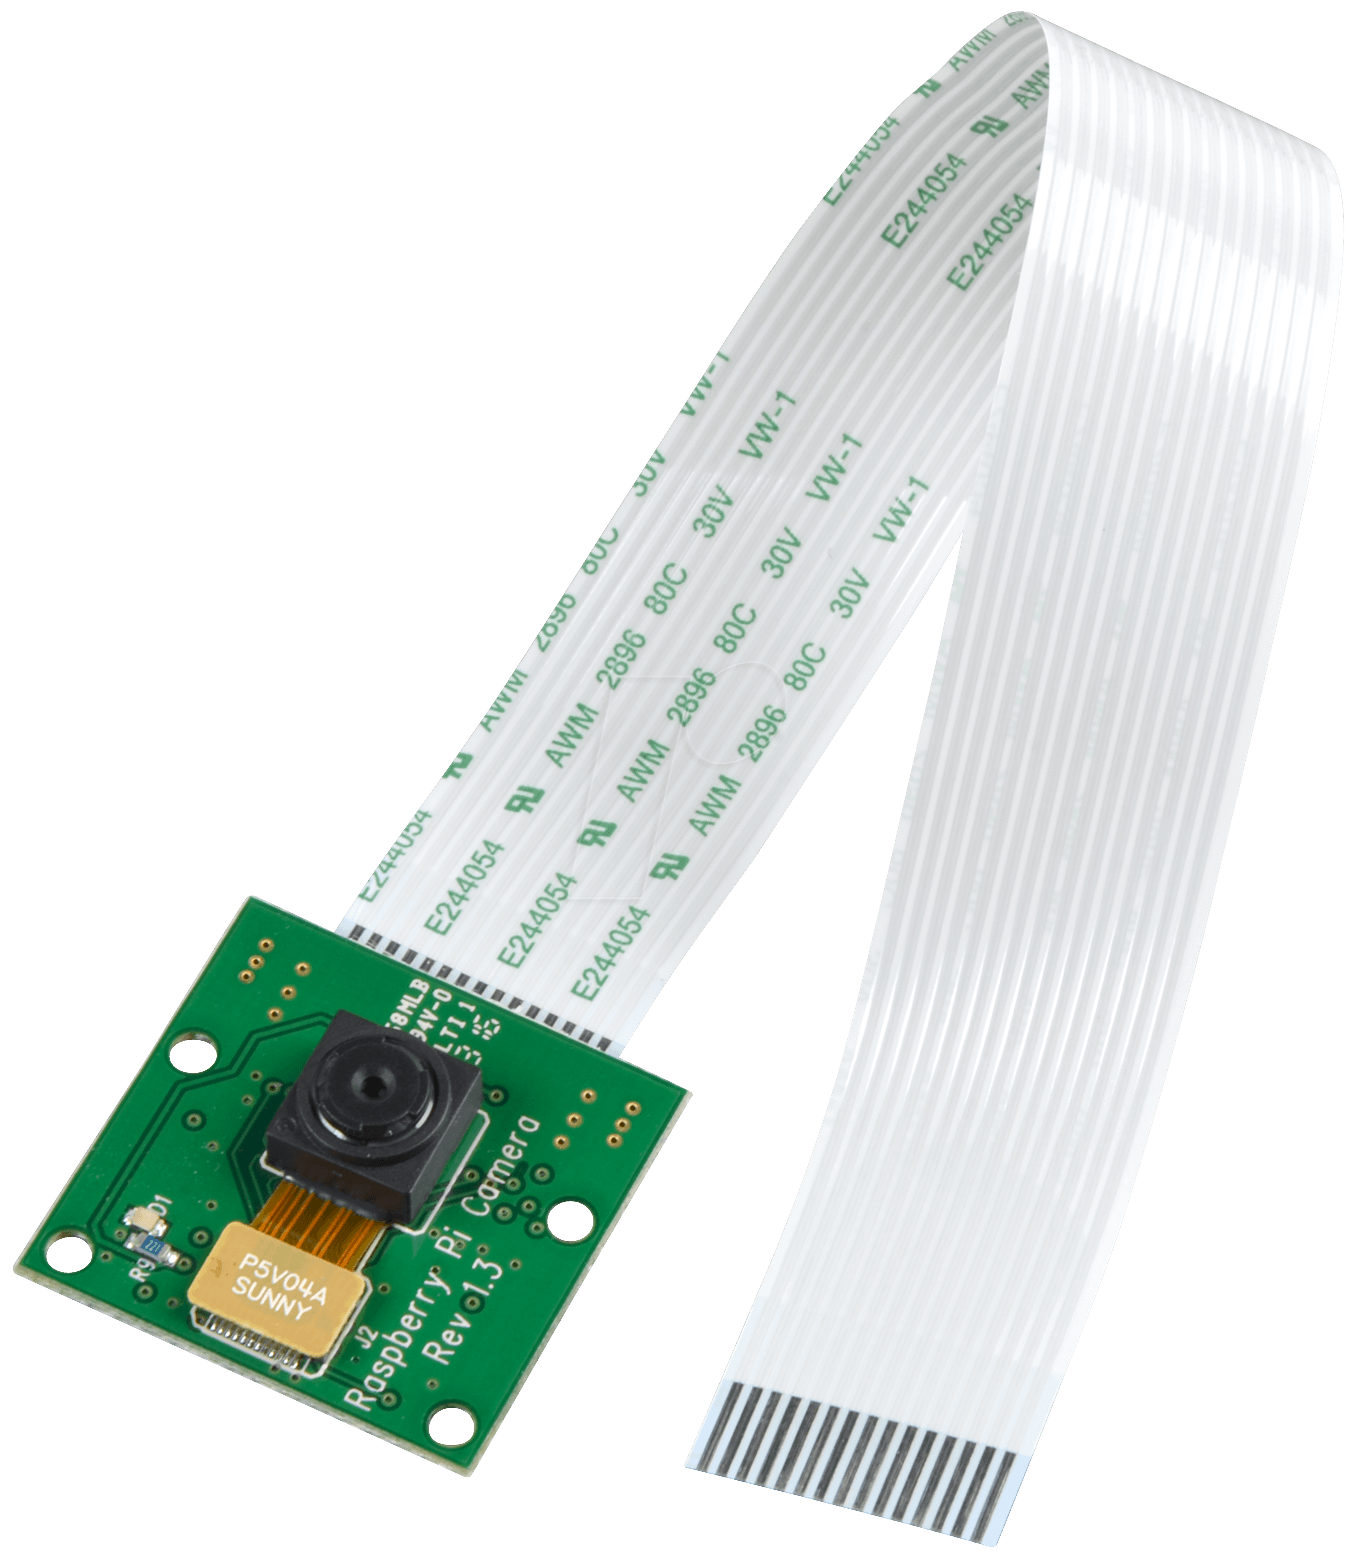
\includegraphics[angle=90,width=0.3\linewidth]{../../fig/raspberry_pi_cam}
\caption{Raspberry Pi Kamera Modul}
\label{fig:raspberry_pi_cam}
\end{figure}
